
\label{subsec:ANN:NARX}

Based on the linear ARX models, NARX ones have been demonstrated 
suitable for modeling nonlinear systems. Its defining general 
equation is
\begin{equation}
\begin{split}
y(t) &=f(y(t-1),y(t-2),...,y(t-n_{a}), \\
&x(t-n_{k}),x(t-(n_{k}+1)),...,x(t-(n_{k}+n_{b})))
\end{split}
\end{equation}
where the next value of the dependent output signal $y(t)$ is 
regressed on the $n_{a}$ previous values of the same output signal 
and $n_{b}$ previous values of the independent exogenous input 
signal $x(t)$. The prediction horizon $n_{k}$ is defined as the 
shift among corresponding input and output values so that current 
input is used for predicting the output in $n_{k}$ time steps in the 
future. The unique dissimilarity with the ARX models lies in the 
non-linearity of the function $f$. \figref{narx} shows a schematic
version of a NARX network.

\begin{figure}[!ht]
\centering
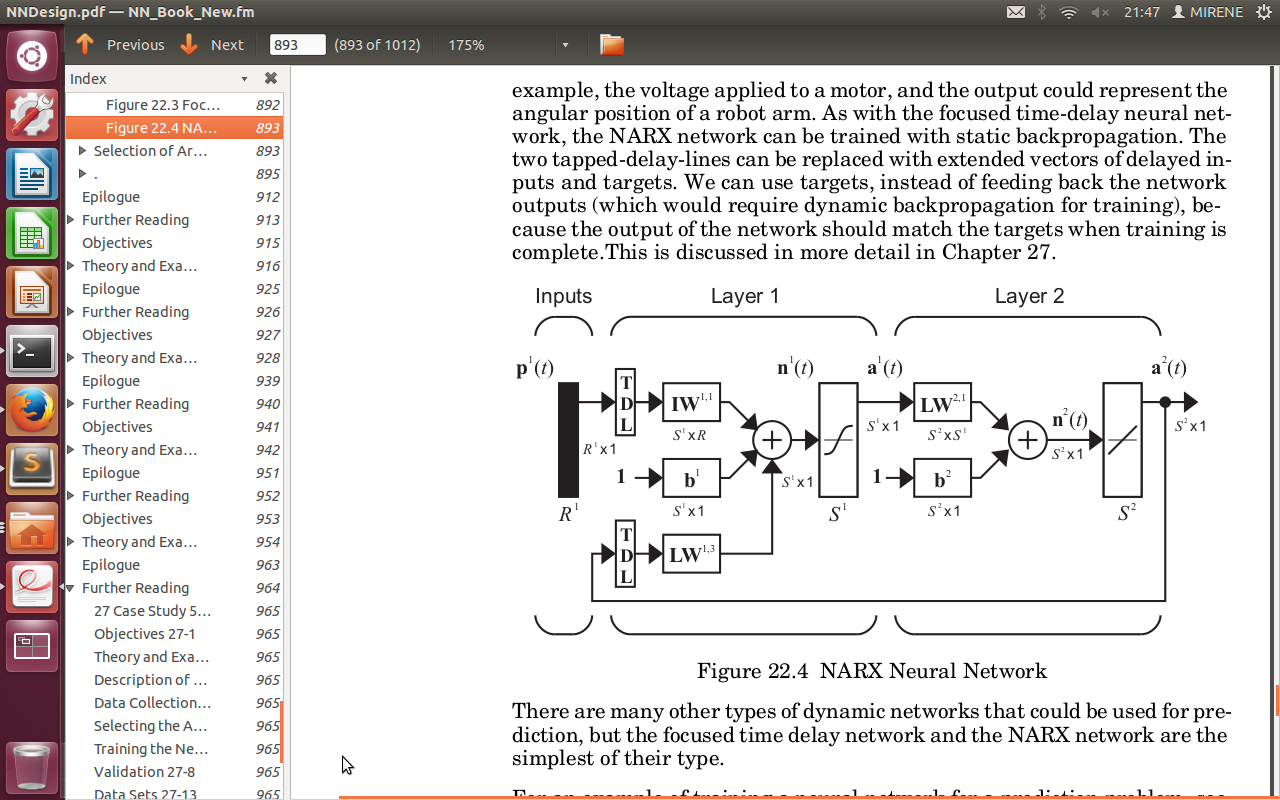
\includegraphics[width=\textwidth]{images/narx.png}
\caption{NARX network}
\label{fig:narx}
\end{figure}



